% Created 2023-05-10 Wed 14:49
% Intended LaTeX compiler: pdflatex
\documentclass[9pt, b5paper]{article}
\usepackage{xeCJK}
\usepackage[T1]{fontenc}
\usepackage{bera}
\usepackage[scaled]{beraserif}
\usepackage[scaled]{berasans}
\usepackage[scaled]{beramono}
\usepackage[cache=false]{minted}
\usepackage{xltxtra}
\usepackage{graphicx}
\usepackage{xcolor}
\usepackage{multirow}
\usepackage{multicol}
\usepackage{float}
\usepackage{textcomp}
\usepackage{algorithm}
\usepackage{algorithmic}
\usepackage{latexsym}
\usepackage{natbib}
\usepackage{geometry}
\geometry{left=1.2cm,right=1.2cm,top=1.5cm,bottom=1.2cm}
\usepackage[xetex,colorlinks=true,CJKbookmarks=true,linkcolor=blue,urlcolor=blue,menucolor=blue]{hyperref}
\newminted{common-lisp}{fontsize=\footnotesize} 
\author{deepwaterooo}
\date{\today}
\title{ET 框架拖拉机项目试改装}
\hypersetup{
 pdfauthor={deepwaterooo},
 pdftitle={ET 框架拖拉机项目试改装},
 pdfkeywords={},
 pdfsubject={},
 pdfcreator={Emacs 28.2 (Org mode 9.5.5)}, 
 pdflang={English}}
\begin{document}

\maketitle
\tableofcontents


\section{双副牌双升108 张卡牌游戏}
\label{sec:org64be5ab}
\begin{itemize}
\item 【游戏可试玩程序】:放在Release/Tractor.exe. Windows 用户大家可以下载试玩儿体验一下。
\item 昨天晚上找见了别人几年前就开发出来的卡五星麻将,所以写麻将游戏的想法就被恶杀在摇篮中。现在再写什么好呢?就只能写【双升拖拉机】了,就是两副牌108 张来打的拖拉机。现已经 ios iPhone 上有的双升游戏,可能搜索一下设计,写安卓版的双升了,看下能否套用ET 框架,写成四人网络【客户端与服务器双热更新的】网络游戏
\item 现在先搜索必要的框架设计,出版规则比大小算法之类的。
\item 【服务器与客户端的同步】:尤其是在分四人牌后,亮主拖底的时候,谁先亮,亮什么主,顺序重要,结果重要。【 ET 框架有专用的游戏服,由游戏服来状态同步】在本程序中,采用的是服务器保存所有的状态,处理所有的逻辑。比如,客户端在点击亮主后,做的事情就是发一个消息给服务器,不做任何显示操作,等待服务器传来亮主的消息后再显示
\begin{itemize}
\item 【发牌,公正性】:随机分牌。第一步就是要发牌。需要做到一个完全随机的发牌,就要保证每张牌发到每个玩家手里的概率都是一样的,而且牌的顺序是等概率随机打乱的。程序中采用的是如下的发牌算法(感谢Dr.Light提供):假如有两幅牌,编号从1到108,首先随机选出一个,并且将牌发给玩家,然后将这个编号的牌与108号牌交换编号,那么剩下的牌就是从1到107号。于是再从中选出一个,重复以上的过程,这样一来,算法的复杂度就是O(n)。
\end{itemize}
\end{itemize}
\section{主要想要改进的地方:前辈十年前开发出的游戏,游戏整体【差强人意】}
\label{sec:org697a571}
\begin{itemize}
\item \textbf{【界面设计:】} 八十年前没有ET 框架,不知道原作者是如何设计这个游戏的。感觉游戏的整体走桌面游戏风,要把菜单设计等改成【手游风格】。
\item \textbf{【逻辑设计,用户意愿:】} 不【尊重用户游戏配置选择】的游戏,永远是固执不受欢迎的。【游戏逻辑、玩法】需要能够给用户留足选择配置空间,如下:
\end{itemize}
\begin{center}
\begin{tabular}{ll}
\textbf{2 为常主} & 是常主,就常主会比较多,否则常主少,尤其打王的时候\\
\textbf{5 10 K 必打} & 因为比较难打\\
\textbf{单 J 勾到6, 双 JJ 勾到 2} & 开历史倒车,增加游戏的无穷乐趣:惊险刺激:逢对家对J, 谁不想把对方废到6 或是2?\\
 & 逢自家打到J, 会想要被对方废到6 或是2?\\
\textbf{逢 J 必打} & 因为上面不能言说的【惊险刺激】,不给任何双方逃跑的好玩机会\\
\textbf{小光升1 级,大光连升3 级} & 不满 40 算小光,0 分为大光头。。。连升三级\\
\textbf{捡分方扣底,底分翻倍} & 单扣乘2, 又扣乘 4, 拖拉机扣牌数乘 2.\\
 & 如此,才能让捡分方快速超越,以风马牛不能及之势火箭升级。。。\\
\end{tabular}
\end{center}
\begin{itemize}
\item 其它这里没有列出来的,主要是我现在还不曾了解那些是在说什么,比如下面网络上提到过的:提供六种配置选项: \textbf{【允许自反】,允许对家保,允许反无将,A 必打} (是为什么呢,K 易跑光,不好捡分?)等
\item \textbf{【点击触屏、用户交互的性能优化】} :需要优化。玩家就算玩得不久,一直点鼠标,也是痛苦的事。需要AI 辅助,智能帮助用户出牌,让鼠标点击、选牌聪敏、反应快。
\item \textbf{【逻辑设计,用户意愿:】}: 逻辑上,为能实现以上种种好玩玩法,游戏逻辑需要 \textbf{规定,约束严格的反牌规则:从高到低为【王黑红梅方】} ,就是别人叫方块的主,其它都可以反,但若是已经反到黑桃,接下来就只能反王或说是常主。允许捡分方按照以上规则反牌,这样才给给予捡分方底牌放 80 分,拖拉机扣底,火箭升级的机会。规则明确,公正。现游戏中一个【“流局”】界面,抹杀了这一切好玩儿的过程与结果,太不好玩了。。。游戏界面,也需要必要的文字提示等,帮助玩家理解游戏中的这些好玩儿规则,让玩家上瘾。。。
\end{itemize}
\section{游戏整体【差强人意】现游戏试玩中抓到的【BUG:】如下}
\label{sec:orgddceb69}
\begin{itemize}
\item 不考虑现代大型网络游戏的双端热更新机制。现在游戏的热更新实在是必备。游戏整体,逻辑相对完整,提供了完整的AI 辅助,主要只是提供了 \textbf{牌面的背景图、游戏桌面背景图、背景音效等配置} 。但 \textbf{游戏逻辑单一固定,不好玩。}
\item 对游戏整体的玩家用户体验如此,但并不是说我就真的狠懂这个游戏项目。实际上,我还没能真正学习这个项目,甚至它底层的算法动态库的连接等,都是我需要从这个十年前的项目中学习的地方。借他山之石,为自己的游戏所用。
\item 现在抓到的主要 bug 如下截图:
\end{itemize}

\begin{center}
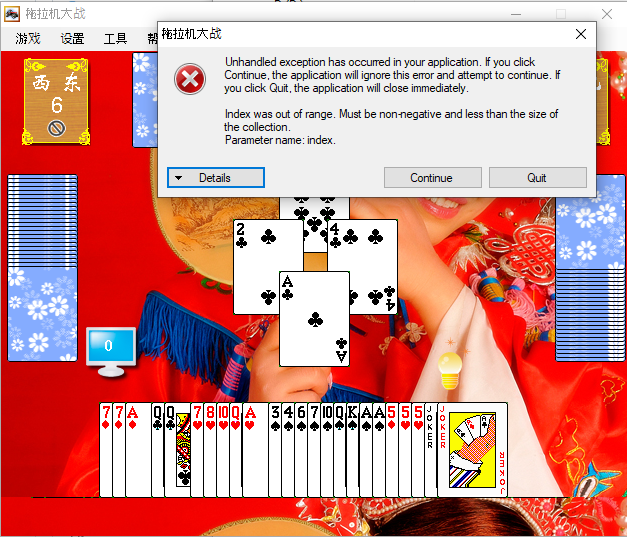
\includegraphics[width=.9\linewidth]{./pic/readme_20230509_230111.png}
\end{center}

\begin{center}
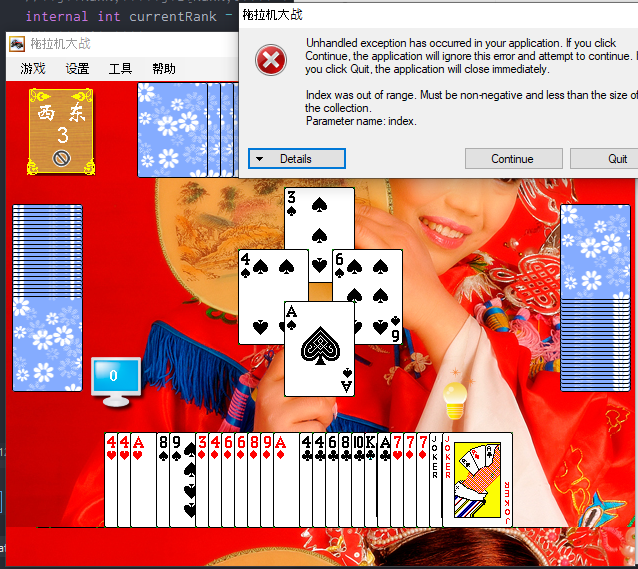
\includegraphics[width=.9\linewidth]{./pic/readme_20230509_232252.png}
\end{center}

\begin{center}
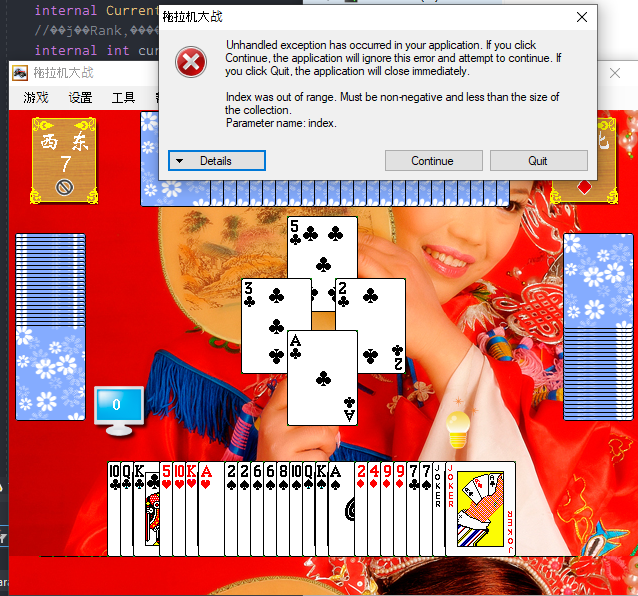
\includegraphics[width=.9\linewidth]{./pic/readme_20230510_014418.png}
\end{center}

\begin{center}
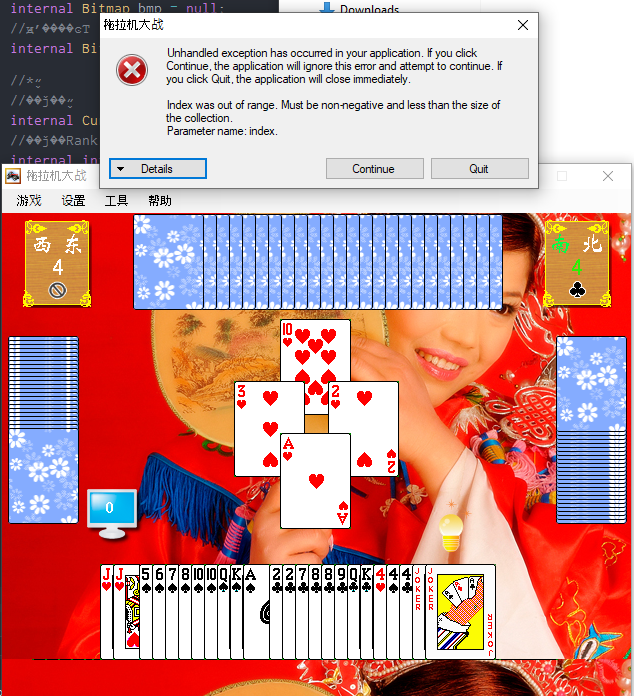
\includegraphics[width=.9\linewidth]{./pic/readme_20230510_015324.png}
\end{center}

\begin{center}
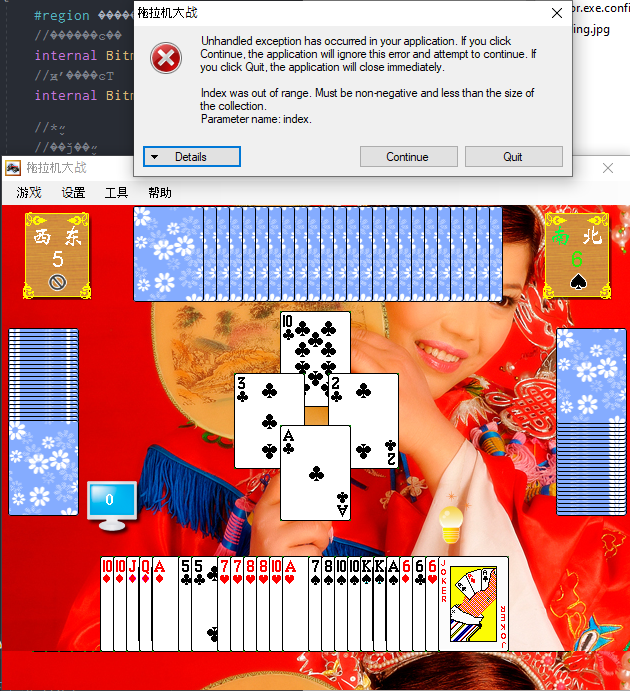
\includegraphics[width=.9\linewidth]{./pic/readme_20230510_033444.png}
\end{center}

\begin{center}
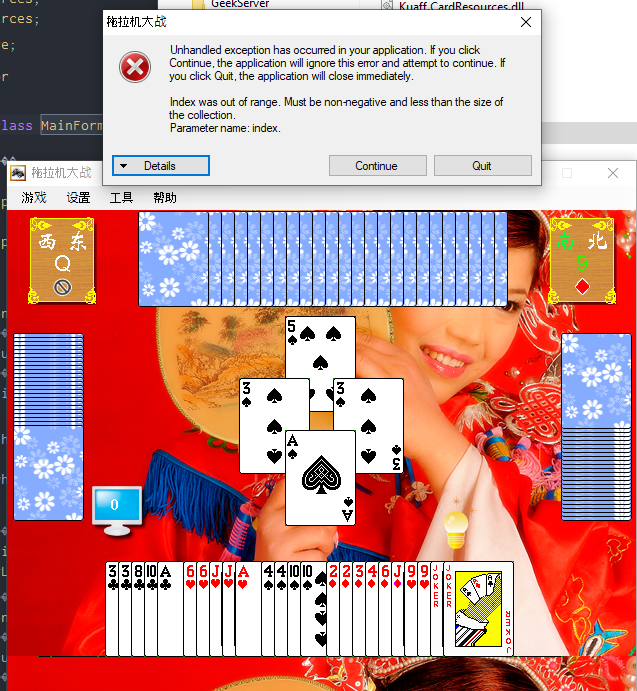
\includegraphics[width=.9\linewidth]{./pic/readme_20230510_042818.png}
\end{center}

\begin{center}
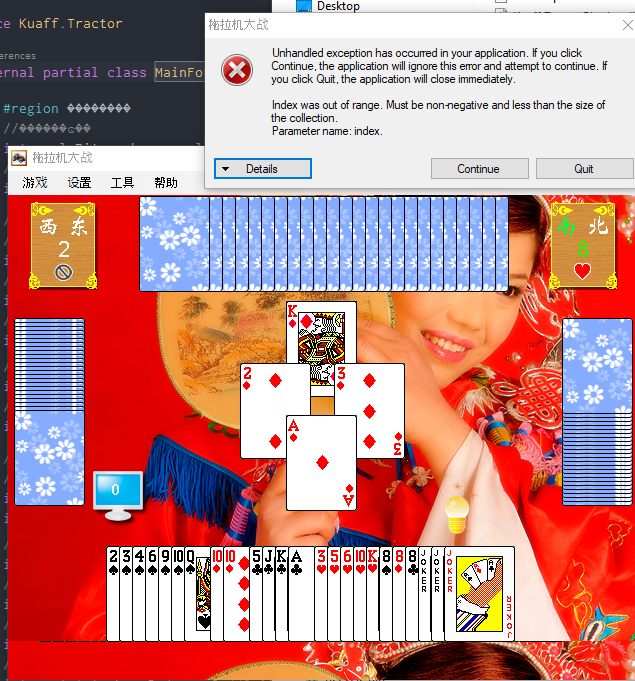
\includegraphics[width=.9\linewidth]{./pic/readme_20230510_043722.png}
\end{center}

\begin{itemize}
\item 【牌的逻辑OOD/OOP】设计:三个类,对应单张,拖拉机(对子是长度为1 的拖拉机),和混合单张与拖拉机
\item 简易版设计原理:模拟拖拉机(升级)玩法;
\begin{itemize}
\item 1.创建两副牌的集合:HashMap
\item 2.创建纸牌:四个花色共108张♦ ♣ ♥ ♠
\item 3.创建poker的ArrayList操作集合
\item 4.创建亮主牌的操作
\item 5.将所有牌放入牌盒中
\item 6.创建四个玩家与底牌的集合:HashSet wj1,wj2,wj3,wj4,dipai
\item 7.洗牌
\item 8.发牌操作
\item 9.创建看牌方法
\item 10.调用方法看牌
\end{itemize}
\item 安桌上的游戏现在是这样的:还要再写一个吗?【活宝妹就是一定要嫁给亲爱的表哥!!!】还是说更为完善或是好玩儿的游戏逻辑?或是UI 视图画面,或是性能表现?反正一定是套用ET 框架写得最容易快速方便。【感觉现在这个截图的UI 长得有点儿丑怪。。】不好看不经典,看了就不想玩儿了。。
\item 因为各处的游戏规则不一样,所以给玩家多点儿自由,自己选择玩法。提供六种配置选项:【允许自反】,允许对家保,2 为常主,允许反无将,五十K 必打,JA 必打等
\end{itemize}
\end{document}